\begin{frame}[t]
  \frametitle{\emph{A priori} estimates}
    If $u \in H^{k+1}(\Omega)$ and $V_h = P^k(\mcT_h)$ then
    \begin{gather*}
      \tn u - u_h \tn \leqslant C h^{k} \| u \|_{\Omega, k+1} \\
      \| u - u_h \|_{L^2(\Omega)} \leqslant C h^{k+1} \| u \|_{\Omega, k+1}
    \end{gather*}
  \begin{columns}[c]
    \begin{column}{0.4\textwidth}
    \multiinclude[graphics={width=1.0\textwidth},format=png]{png/mesh-ref}
    \end{column}
    \begin{column}{0.6\textwidth}
    \only<2>{
      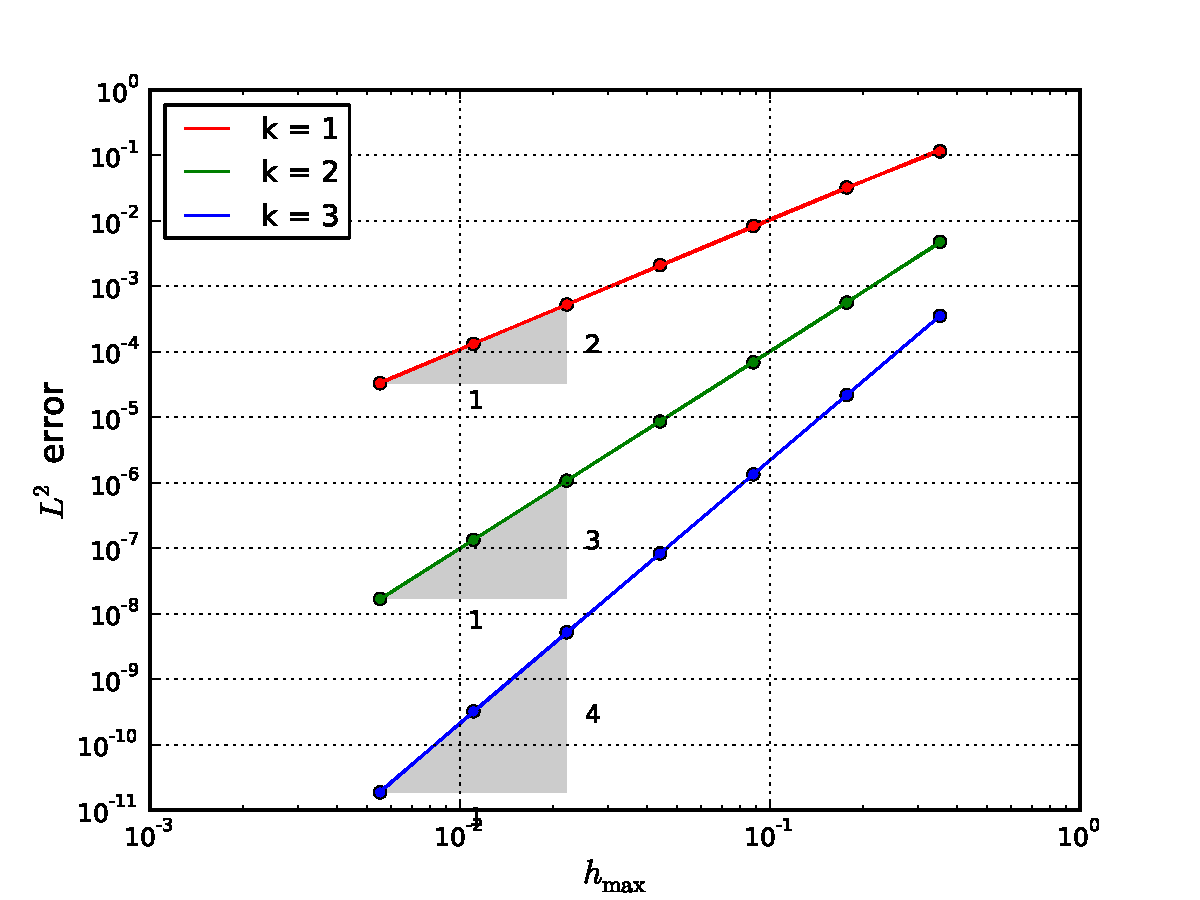
\includegraphics[width=1.0\textwidth]{pdf/l2-convergence.pdf}
    }
    \only<3>{
      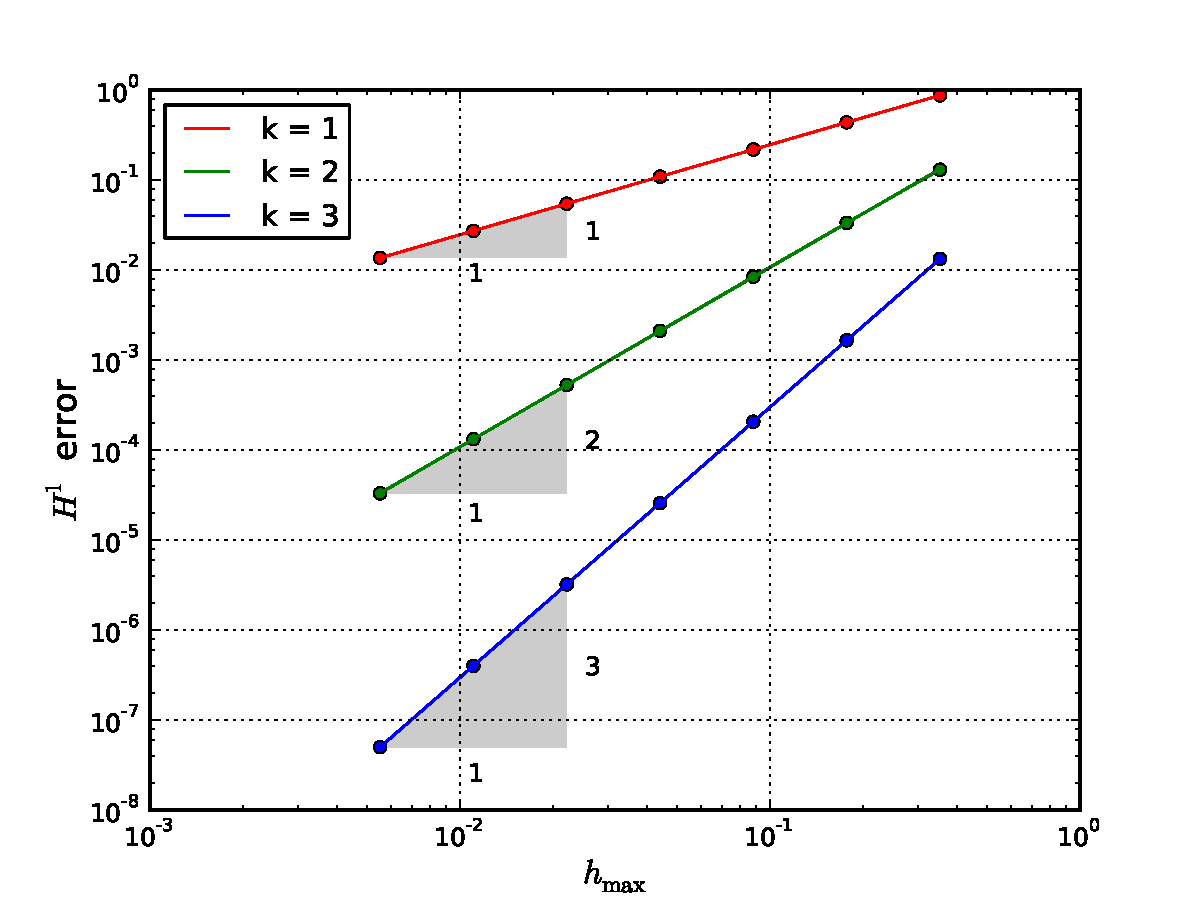
\includegraphics[width=1.0\textwidth]{pdf/h1-convergence.pdf}
    }
    \end{column}
  \end{columns}
%Figure left: mesh refinement \\
%Figure right: convergence plots for p = 1 2 3 \\
%Mention h vs p vs hp estimates. Mention paper by rivere ..
\end{frame}
